\begin{figure}[h!]
	\centering{
		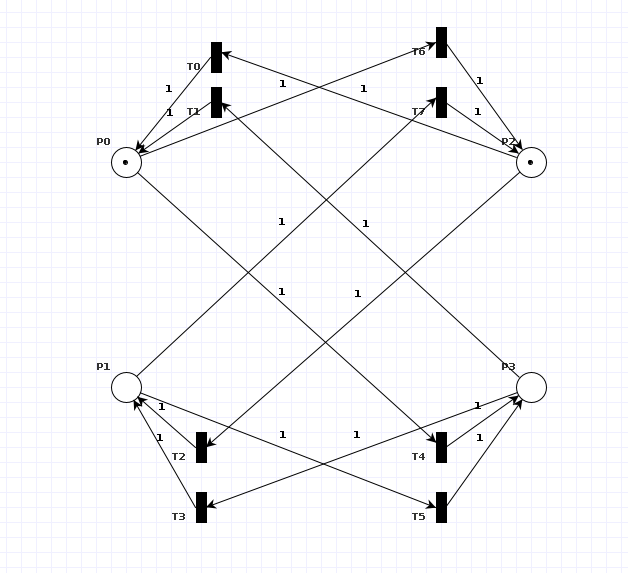
\includegraphics[width=0.67\textwidth]{img/bipartite.png}
	}
	\caption{Maszyna stanów}
	\label{zad2:graph1}
\end{figure}

\begin{figure}[h!]
	\centering{
		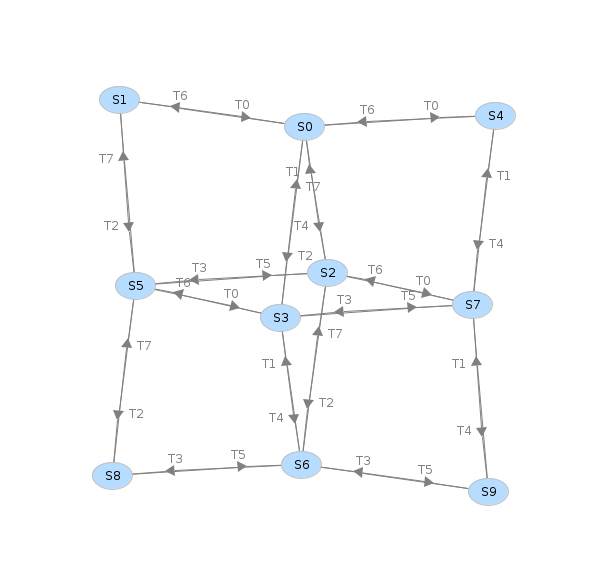
\includegraphics[width=0.67\textwidth]{img/bipartiteg.png}
	}
	\caption{Graf osiągalności maszyny stanów}
	\label{zad2:graph1}
\end{figure}

\subsection{Analiza grafu osiągalności}
\begin{itemize}
	\item Jak widać na grafie osiągalności - wszystkie stany są osiągalne.
	\item Sieć jest zachowawcza i $2$ - ograniczona, ale nie jest bezpieczna.
	\item Każde przejście jest krawędzią w grafie.
	\item Sieć jest żywa.
\end{itemize}


\subsection{Analiza niezmienników}
\quad Wiemy, że wszystkie możliwe rozkłady dwóch zasobów sieci są osiągalne. 
Więc jedynym niezmiennikiem miejsc jest $P_0 + P_1 + P_2 + P_3 = 2$, mówiący nam o tym, że 
sieć jest zachowawcza.

Podobna sytuacja z niezmiennikami przejść. Możemy wrócić do stanu początkowego przez 
dowolną krawędź w dwóch krokach.